\documentclass[../../LearnCpp.tex]{subfiles}

\begin{document}

\asubsection{6}{The virtual table}

为了实现虚函数,C++ 使用了一种被称为虚表的特别形式的 late binding。
\textbf{虚表} virtual table 是一个检索函数的表,用于在动态/late binding 情况下解析函数调用。
虚表有时会有别的名字,例如“vtable”,“virtual function table”,“virtual method table”,或者“dispatch table”。

虚表实际上非常简单,尽管用文字表达起来会有些复杂。
首先,每个使用了虚函数的类(或是使用虚函数的派生类)都会被给予自身的虚表。
这个表是一个由编译器在编译时设置好的静态数组。
虚表包含了每个可以被类对象所调用的虚函数的入口。
每个入口就是一个函数指针,其指向的是类可以访问到的最-派生的函数。

其次,编译器添加一个身为基类成员的隐藏指针,其可以称为 \acode{*\_\_vptr}。
当类对象被创建时, \acode{*\_\_vptr} 被自动设置,因此它可以指向该类的虚表。
不同于 \acode{*this} 指针,即实际上是一个函数参数用作于编译器解析自引用,\acode{*\_\_vptr} 是一个真实指针。结果而言,它使得每个类对象分配的大小都会大于一个指针。这同样也意味着 \acode{*\_\_vptr} 是会继承给派生类,这点非常重要。

现在来看一个例子:

\begin{lstlisting}[language=C++]
class Base
{
public:
    virtual void function1() {};
    virtual void function2() {};
};

class D1: public Base
{
public:
    void function1() override {};
};

class D2: public Base
{
public:
    void function2() override {};
};
\end{lstlisting}

上述有 3 个类,编译器会设置 3 个虚表: \acode{Base},\acode{D1} 以及 \acode{D2}。

编译器同时添加了隐藏指针成员给使用虚函数的基类。
尽管编译器自动化了这个步骤,在下一个例子中展示它添加在哪里:

\begin{lstlisting}[language=C++]
class Base
{
public:
    VirtualTable* __vptr;
    virtual void function1() {};
    virtual void function2() {};
};

class D1: public Base
{
public:
    void function1() override {};
};

class D2: public Base
{
public:
    void function2() override {};
};
\end{lstlisting}

当一个类对象被创建,\acode{*\_\_vptr} 被设置指向该类的虚表。
例如,当一个 Base 类型的对象被创建,\acode{*\_\_vptr} 被设置指向 \acode{Base} 的虚表。
当 \acode{D1} 或 \acode{D2} 类型的对象被构建,\acode{*\_\_vptr} 则分别被设置指向它们各自的虚表。

那么现在来看一下这些虚表是如何被填充的。
因为这里只有两个虚函数,每个虚表都会有两个入口(一个是 \acode{function1()} 另一个是 \acode{function2()})。
当这些虚表被填充,每个入口都会填充该类对象所能调用的最-派生的函数。

\acode{Base} 对象的虚表很简单。
\acode{Base} 类型的对象仅可以访问 \acode{Base} 的成员。
\acode{Base} 不能访问 \acode{D1} 或 \acode{D2} 的函数。
结果而言,\acode{function1} 的入口指向 \acode{Base::function1()} 同时 \acode{function2} 的入口指向 \acode{Base::function2()}。

\acode{D1} 的虚表会稍微复杂一些。
\acode{D1} 类型的对象可以访问 \acode{D1} 与 \acode{Base} 的成员。
然而,\acode{D1} 拥有重写函数 \acode{function1()},使得 \acode{D1::function1()} 比 \acode{Base::function1()} 更-派生一些。
结果,\acode{function1} 的入口指向了 \acode{D1::function1()}。
\acode{D1} 没有重写 \acode{function2()},因此 \acode{function2} 的入口指向 \acode{Base::function2()}。

\acode{D2} 与 \acode{D1} 类似,不再赘述。

\begin{figure}[h]
    \centering
    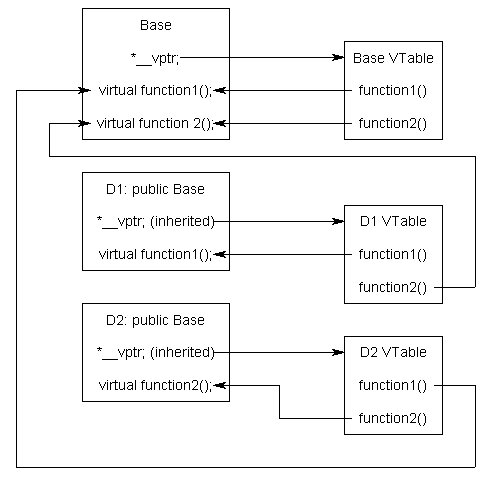
\includegraphics[width=10cm]{\subfix{../images/VTable}}
    \label{fig:VTable}
    \caption{VTable}
\end{figure}

经过上图看起来很复杂,但是实际上非常简单:
每个类中的 \acode{*\_\_vptr} 指向该类自身的虚表。
虚表中的入口指向了该类对象可以调用的最-派生版本的函数。

考虑一下创建了 \acode{D1} 类型对象会发生什么:

\begin{lstlisting}[language=C++]
int main()
{
    D1 d1;
}
\end{lstlisting}

由于 \acode{d1} 是 \acode{D1} 对象,其拥有的 \acode{*\_\_vptr} 设置到 \acode{D1} 虚表。

现在设置一个 \acode{D1} 的基类指针:

\begin{lstlisting}[language=C++]
int main()
{
    D1 d1;
    Base* dPtr = &d1;

    return 0;
}
\end{lstlisting}

注意因为 \acode{dPtr} 是一个基类指针,它仅指向了 \acode{d1} 的 \acode{Base} 部分。
然而同样注意 \acode{\_\_vptr} 也在 \acode{Base} 部分,因此 \acode{dPtr} 可以访问到这个指针。
最后就是注意 \acode{dPtr->\_\_vptr} 指向 \acode{D1} 虚表!
结果,即使 \acode{dPtr} 是 \acode{Base} 类型,它仍然能访问 \acode{D1} 虚表(通过 \acode{\_\_vptr})。

那么当尝试调用 \acode{dPtr->function1()} 会发生什么呢?

\begin{lstlisting}[language=C++]
int main()
{
    D1 d1;
    Base* dPtr = &d1;
    dPtr->function1();

    return 0;
}
\end{lstlisting}

首先程序会察觉 \acode{function1()} 是一个虚函数。
其次,程序使用 \acode{dPtr->\_\_vptr} 来获取 \acode{D1} 的虚表。
第三,查看 \acode{D1} 中需要调用哪个版本的 \acode{function1()}。
这里是 \acode{D1::function1()}。
因此 \acode{dPtr->function1()} 解析成为 \acode{D1::function1()}。

但是有人可能会说“如果 \acode{dPtr} 指向的是 \acode{Base} 对象而不是 \acode{D1} 对象,
还会调用 \acode{D1::function1()} 吗?”。答案是不。

\begin{lstlisting}[language=C++]
int main()
{
    Base b;
    Base* bPtr = &b;
    bPtr->function1();

    return 0;
}
\end{lstlisting}

这个情况中,当 \acode{b} 被创建,\acode{\_\_vptr} 指向的是 \acode{Base} 的虚表,
而不是 \acode{D1} 的虚表。
结果就是 \acode{bPtr->\_\_vptr} 同样指向 \acode{Base} 的虚表,
其 \acode{function1()} 的入口指向 \acode{Base::function1()}。
因此,\acode{bPtr->function1()} 解析为 \acode{Base::function1()},
即对于一个 \acode{Base} 对象而言,可以调用的最-派生的 \acode{function1()} 版本。

\end{document}
